\documentclass[12pt]{article}

% Layout.
\usepackage[top=1in, bottom=0.75in, left=1in, right=1in, headheight=1in, headsep=6pt]{geometry}

% Fonts.
\usepackage{mathptmx}
\usepackage[scaled=0.86]{helvet}
\renewcommand{\emph}[1]{\textsf{\textbf{#1}}}

% TiKZ.
\usepackage{tikz, pgfplots}
\usetikzlibrary{calc}
\usetikzlibrary{calc,trees,positioning,arrows,fit,shapes,through, backgrounds}
\usetikzlibrary{patterns}

\usetikzlibrary{decorations.markings}
\usetikzlibrary{arrows}

\usepackage{pgfplots}

\usepackage{longtable}
\usepackage{tabularx}


% Misc packages.
\usepackage{amsmath,amssymb,latexsym}
\usepackage{graphicx}
\usepackage{array}
\usepackage{xcolor,enumerate, tabularx,adjustbox}
\usepackage{multicol}
\usepackage{fancyhdr}
\pagestyle{fancy}


% Misc.
\renewcommand{\d}{\displaystyle}
\newcommand{\ds}{\displaystyle}
\newcommand{\ul}[1]{\underline{#1}}
\def\bc{\begin{center}}
\def\ec{\end{center}}
\def\be{\begin{enumerate}}
\def\ee{\end{enumerate}}

\newcommand{\ans}[1][1in]{\rule{#1}{.5pt}}


\lhead{Exam II Review}
\rhead{Spring 2025}

\begin{document}
\begin{center} {\Large{Graph Theory}} \end{center}
\begin{enumerate}
\item Define the terms below.
	\begin{enumerate}
	\item An Euler circuit is 
	\vfill
	\item An Euler path is
	\vfill
	\item A Hamiltonian circuit is
	\vfill
	\item A spanning tree is
	\vfill
	\end{enumerate}
\item 
	\begin{enumerate}
	\item Use Kruskal's Algorithm to find a minimum weight spanning tree in the graph below.\\
	
	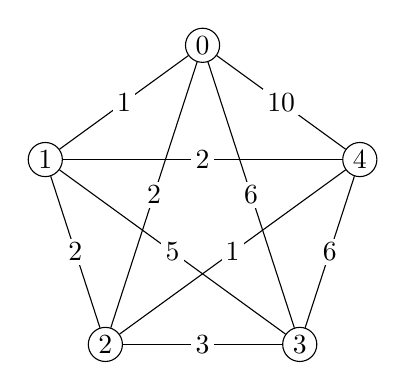
\begin{tikzpicture}[vtx/.style={draw, circle, inner sep =1.5 pt}, lbl/.style =  {inner sep =1.5 pt, fill = white},scale=.7]
\foreach \i in {0,1,2,3,4}{\node[vtx] (\i) at (360*\i/5+90:3){\i};}
\foreach \i in {0,1,2,4}{\draw let \n1 = {int(mod(\i+1, 5))}, \n2 = {int(2*\i-1*\n1+2)}
 in (\i) -- node[lbl] {\n2} 
(\n1);}
\foreach \i in {0,1,2,4}{\draw let \n1 = {int(mod(\i+2, 5))}, \n2 = {int(mod(2*\i+1*\n1,7))}
in (\i) -- node[lbl] {\n2} 
(\n1);}
\draw (3) -- node[lbl] {6} (0);
\draw (3) -- node[lbl] {6} (4);
\end{tikzpicture}
\hfill
\begin{tikzpicture}[vtx/.style={draw, circle, inner sep =1.5 pt}, lbl/.style =  {inner sep =1.5 pt, fill = white},scale=.7]
\foreach \i in {0,1,2,3,4}{\node[vtx] (\i) at (360*\i/5+90:3){\i};}
\end{tikzpicture}
	\vfill
	\item Give an example of a real-world problem which you would want to find a minimum weight spanning tree. (You would need to state what are the vertices, edges, and weights!)
	\vfill
	\end{enumerate}
\newpage
\item 
	\begin{enumerate}
	\item Use Dijkstra's Algorithm to find the distance of each vertex from vertex $S.$.\\
	
	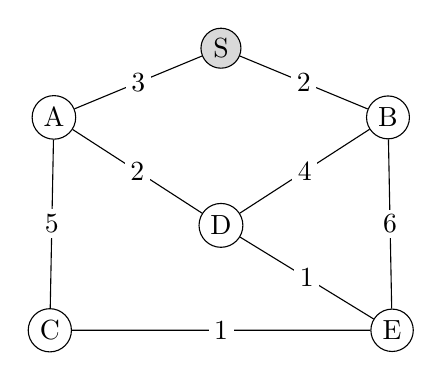
\begin{tikzpicture}[baseline=(current bounding box.center),lbl/.style={inner sep = 2pt, fill = white}, scale = 1.5]
\tikzstyle{vtx}=[circle, draw, inner sep=2pt]
\node[vtx, fill = gray!30] (S) at (90:2) {S};
\node[vtx] (A) at (135:2) {A};
\node[vtx] (B) at (45:2) {B};
\node[vtx] (D) at (90:0.5){D};
\node[vtx] (C) at (15+180:1.5){C};
\node[vtx] (E) at (-15:1.5){E};
\foreach \i/\j/\k in {S/A/3,S/B/2,A/C/5, A/D/2,B/D/4,B/E/6,C/E/1,E/D/1}{\draw (\i) --node[lbl]{\k} (\j);}
\end{tikzpicture}

\begin{minipage}[t]{.6\linewidth}
\begin{tabular}{ c | c | p{1.5in}}
Explored? & vertices & tentative distances\\ \hline
&S& \\[12pt] \hline
&A& \\[12pt]\hline
&B& \\[12pt]\hline
&C& \\[12pt]\hline
&D& \\[12pt]\hline
&E& \\[12pt]\hline
 \end{tabular}

 \end{minipage}
% 
\vspace{1cm}
%
 %
 \begin{minipage}{.4\linewidth}
 \begin{tabular}{ c | p{.8in} }
 vertex & minimum distance to S\\ \hline
S& \\[12pt] \hline
A& \\[12pt]\hline
B& \\[12pt]\hline
C& \\[12pt]\hline
D& \\[12pt]\hline
E& \\[12pt]\hline \end{tabular}
 \end{minipage}
\vfill

	
	\vfill
	\item Give an example of a real-world problem which you would want to find the minimum distance from $S.$ (You would need to state what are the vertices, edges, and weights!)
	\vfill
	\end{enumerate}
\newpage
\item 
	\begin{enumerate}
	\item What does it mean to Eulerize a graph? What is your goal?
	\vfill
	\item Eulerize the graph below by adding the fewest number of edges and then find an Euler circuit in the resulting graph.\\
	
	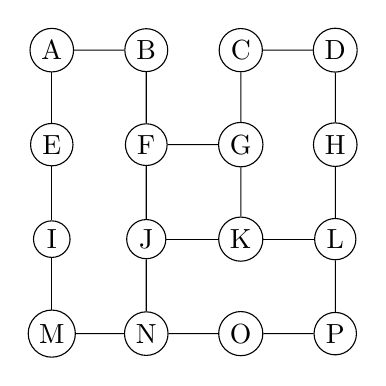
\begin{tikzpicture}[baseline=(current bounding box.center),lbl/.style={inner sep = 2pt, fill = white}, scale = 1.2]
\tikzstyle{vertex}=[circle, draw, inner sep=2pt]
\tikzstyle{every node} = [vertex];
\node (a) at (0,2) {A};
\node (b) at (1,2) {B};
\node (c) at (2,2) {C};
\node (d) at (3,2) {D};
\node (e) at (0,1) {E};
\node (f) at (1,1){F};
\node (g) at (2,1){G};
\node (h) at (3,1){H};
\node (i) at (0,0) {I};
\node (j) at (1,0) {J};
\node (k) at (2,0) {K};
\node (l) at (3,0) {L};
\node (m) at (0,-1) {M};
\node (n) at (1,-1) {N};
\node (o) at (2,-1) {O};
\node (p) at (3,-1) {P};
\foreach \i/\j in {a/b,c/d,f/g,g/k,j/k,k/l,m/n,n/o,o/p,a/e,b/f,c/g,d/h,e/i,i/m,f/j,h/l,l/p,j/n}{\draw (\i) -- (\j);}
\end{tikzpicture}

	\vfill
	\item Give an example of a real-world problem which you would want to find an Euler circuit. (You would need to state what are the vertices and edges.)
	\vfill
	\end{enumerate}

\newpage
\item 
	\begin{enumerate}
	\item Use the Nearest Neighbor Algorithm starting a vertex $A,$ to find a Hamiltonian Circuit in the graph below and determine its weight.\\
	
	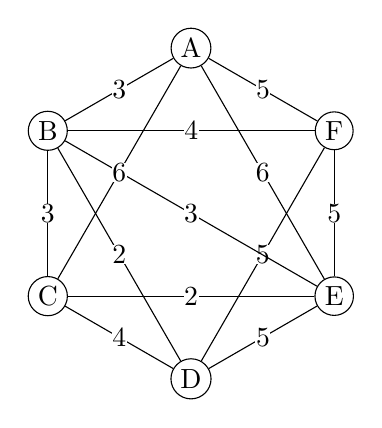
\begin{tikzpicture}[vtx/.style={draw, circle, inner sep =1.5 pt}, lbl/.style =  {inner sep =0.2 pt, fill = white},scale=.7]
\foreach \i/\j in {0/A,1/B,2/C,3/D,4/E,5/F}{\node[vtx] (\i) at (360*\i/6+90:3){\j};}
%edges for 5 or F
\foreach \i/\j in {0/5,1/4,3/5,4/5}{\draw (5) -- node[lbl] {\j} (\i);}
%edges for 4 or E
\foreach \i/\j in {0/6,1/3,2/2,3/5}{\draw (4) -- node[lbl] {\j} (\i);}
%edges for 3 or D
\foreach \i/\j in {1/2,2/4}{\draw (3) -- node[lbl] {\j} (\i);}
%edges for 2 or C
\foreach \i/\j in {0/6,1/3}{\draw (2) -- node[lbl] {\j} (\i);}
%edges for 1 or B
\foreach \i/\j in {0/3}{\draw (1) -- node[lbl] {\j} (\i);}
\end{tikzpicture}
\hfill
\begin{tikzpicture}[vtx/.style={draw, circle, inner sep =1.5 pt}, lbl/.style =  {inner sep =0.2 pt, fill = white},scale=.7]
\foreach \i/\j in {0/A,1/B,2/C,3/D,4/E,5/F}{\node[vtx] (\i) at (360*\i/6+90:3){\j};}
\end{tikzpicture}
	\vfill
	\item Use the Cheapest Link Algorithm to find a minimum weight Hamiltonian Circuit in the graph below.\\
	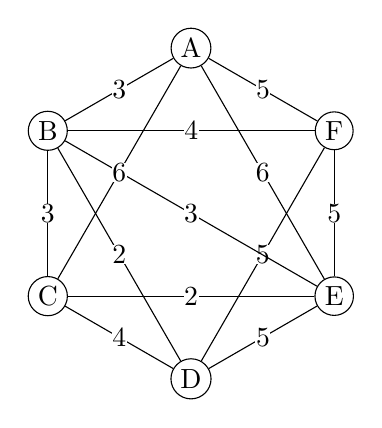
\begin{tikzpicture}[vtx/.style={draw, circle, inner sep =1.5 pt}, lbl/.style =  {inner sep =0.2 pt, fill = white},scale=.7]
\foreach \i/\j in {0/A,1/B,2/C,3/D,4/E,5/F}{\node[vtx] (\i) at (360*\i/6+90:3){\j};}
%edges for 5 or F
\foreach \i/\j in {0/5,1/4,3/5,4/5}{\draw (5) -- node[lbl] {\j} (\i);}
%edges for 4 or E
\foreach \i/\j in {0/6,1/3,2/2,3/5}{\draw (4) -- node[lbl] {\j} (\i);}
%edges for 3 or D
\foreach \i/\j in {1/2,2/4}{\draw (3) -- node[lbl] {\j} (\i);}
%edges for 2 or C
\foreach \i/\j in {0/6,1/3}{\draw (2) -- node[lbl] {\j} (\i);}
%edges for 1 or B
\foreach \i/\j in {0/3}{\draw (1) -- node[lbl] {\j} (\i);}
\end{tikzpicture}
\hfill
\begin{tikzpicture}[vtx/.style={draw, circle, inner sep =1.5 pt}, lbl/.style =  {inner sep =0.2 pt, fill = white},scale=.7]
\foreach \i/\j in {0/A,1/B,2/C,3/D,4/E,5/F}{\node[vtx] (\i) at (360*\i/6+90:3){\j};}
\end{tikzpicture}
	\vfill
	\item Give an example of a real-world problem which you would want to find a minimum weight Hamiltonian circuit. (You would need to state what are the vertices, edges, and weights.)
	\vfill
	\end{enumerate}
\newpage
\begin{center} {\Large{Scheduling}} \end{center}
\item The table below contains the tasks to be completed for a project.\\
\begin{tabular}{| c|c|c|}
\hline
task& time& dependencies/\\
&(in minutes)&prerequisites\\
\hline
A&2&\\ \hline
B&9&\\ \hline
C&3&\\ \hline
D&7&A\\ \hline
E&1&C\\ \hline
F&6&A\\ \hline
G&4&E\\ \hline
H&8&D,F\\ \hline
I&5&G\\ \hline
J&1&B,H,I\\ \hline
\end{tabular}
	\begin{enumerate}
	\item To the right, above, create a digraph representing the project.
	\item Find a critical path and its corresponding critical time. Explain the significance of the critical time.
	\vfill
	\item Create a priority list using the decreasing time algorithm. (That is, create a priority list ordered by decreasing time.)
	\vfill
	\item Use the Backflow algorithm to assign critical numbers to each vertex in the graph above.
	\item Create a priority list using the critical time algorithm. (That is, create a priority list ordered by decreasing \textbf{critical} time.)
	\vfill
	\end{enumerate} 
\newpage
\item Use the diagraph below and the given priority list to construct a schedule using two processors.

\def\r{2}
\def\s{.6}

\begin{tikzpicture}[vtx/.style={draw, circle, inner sep = 3pt, font = \scriptsize}, myto/.style={-latex, shorten >=2pt, shorten <=2pt
}, node distance = \r cm]
\node[vtx, label=above:{\scriptsize $A(10)$}, ] (A) at (0,0){};
\node[vtx, below = \s cm of A, label=above:{\scriptsize $B(5)$}] (B) {};
\node[vtx, below =\s cm of B, label=above:{\scriptsize $F(3)$}] (F) {};
\node[vtx, right = of B, label=above:{\scriptsize $C(4)$}] (C) {};
\node[vtx, right = 2*\r of C, label=above left:{\scriptsize $D(1)$}] (D) {};
\node[vtx, right =of D, label= right:{\scriptsize $E(8)$}] (E) {};
\node[vtx, right = of F, label=below:{\scriptsize $G(1)$}] (G) {};
\node[vtx, right =of G, label=below:{\scriptsize $H(7)$}] (H) {};
\node[vtx, below =\s cm of H, label=below:{\scriptsize $J(6)$}] (J) {};

\foreach \i/\j in {B/C,F/C,F/G,G/H,G/J,C/D,D/E, H/D}{\draw[myto] (\i) -- (\j);}
\end{tikzpicture}

Construct a schedule using the priority list \[F, B, G, C, A, H, J, D, E\]

\begin{tabular}{c | c | c}
time & ready & done \\ \hline
&&\\&&\\&&\\&&\\&&\\&&\\&&\\
\end{tabular}

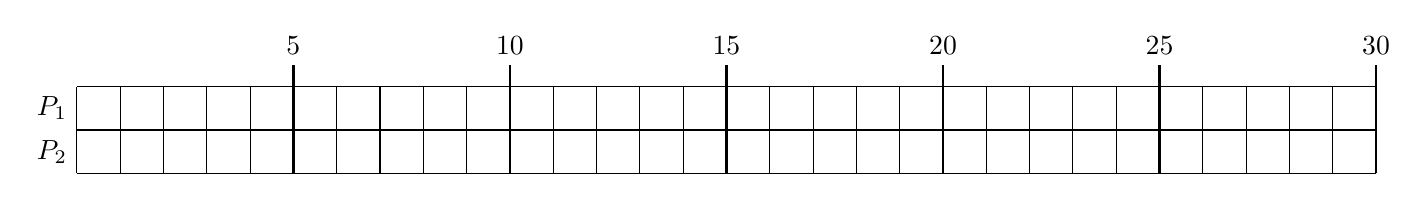
\begin{tikzpicture}[scale = 1.1, lbl/.style={font=\tiny, inner sep = 1 pt, fill = white}]
\path (0, 3/4) node[left] {$P_{1}$};
\path (0, 1/4) node[left] {$P_{2}$};
\draw[step=1/2] (0,0) grid (30/2, 2/2);
\foreach \i in {5, 10, ..., 30}{\draw[thick] (\i/2,0) -- (\i/2,2/2+1/4) node[above]{\i};}
\end{tikzpicture}



 
\end{enumerate}
\end{document}